\documentclass[../main.tex]{subfiles}	

\begin{document}
	
\chapter{Mathematical Proofs}
\label{app:cmplx_optim}


\section{Complex Weights Initialization \cite{trabelsi2018deep}}
\label{app:weight_init}

For complex-valued deep learning traditional approaches of Glorot \cite{xavier_init} and He \cite{he2015delving}, are no more suitable to be used for weights initialization. So we need to re-derive, or at least adapt, those efficient methods also for the complex domain.\\
Given a generic neural network layer, let's call $\vb{w}\in\mathds{C}$ its set of complex-valued weights, that we prefer written in polar form:
\[ \vb{w} = \norm{\vb{w}}e^{i\theta} \]
The variance of this set is defined as 
\[ \Var(\vb{w}) = \Ev{\vb{w}\bar{\vb{w}}} - (\Ev{\vb{w}})^2 = \Ev{\norm{\vb{w}}^2} - (\Ev{\vb{w}})^2 \]
that, if the parameters are symmetrically distributed around 0, reduces to $\Ev{\norm{\vb{w}}^2}$.\\
In order to compute these quantities, we rely on the fact that the magnitude of a standard complex normally distributed variable follows the Rayleigh distribution \footnote{\href{https://en.wikipedia.org/wiki/Rayleigh\_distribution}{Rayleigh Distribution}}, i.e. basically a Chi-Square with two degrees of freedom. Just for knowledge, its probability density function depends only on a single parameter and writes
\[ f(x; \sigma) = \frac{x}{\sigma^2}e^{-x^2 / (2\sigma^2)} \]
So we can find a relation among the variances of $\vb{w}$ and its magnitude:
\[ \Var(\norm{\vb{w}}) = \Var{\vb{w}} - (\Ev{\norm{\vb{w}}})^2 \qquad\longrightarrow\qquad \Var({\vb{w}}) = \Var(\norm{\vb{w}}) + (\Ev{\norm{\vb{w}}})^2 \]
But now, that we know the analytical distribution followed by $\norm{\vb{w}}$, we can derive also the two addends of the sum above:
\[ \Ev{\norm{\vb{w}}} = \sigma\sqrt{\frac{\pi}{2}}, \qquad \Var{\norm{\vb{w}}} = \frac{4-\pi}{2}\sigma^2 \]
The variance of $\vb{w}$ can thus be expressed in terms of its generating Rayleigh distribution's single parameter $\sigma$:
\[ \Var(\vb{w}) = \frac{4-\pi}{2}\sigma^2 + \left(\sigma\sqrt{\frac{\pi}{2}}\right)^2 = 2\sigma^2 \]
How can we determine $\sigma$?\\
\begin{itemize}
	\item Following the Xavier initialization \cite{xavier_init}, we would exploit a normal distribution (or a truncated-normal) with variance $\Var(\vb{w}) = 2 / (n_{in} + n_{out})$, with $n_{in}$ and $n_{out}$ being the number of input and output units, respectively. For continuity, we have now to set
	\[ \sigma = 1 / \sqrt{n_{in} + n_{out}} \]
	\item With the He initialization \cite{he2015delving}, instead, we used still a normal distribution, but with a variance depending only on input units, i.e. $\Var(\vb{w}) = 2/n_{in}$, for which we have to set correspondingly
	\[ \sigma = 1 / \sqrt{n_{in}} \]
\end{itemize}
The magnitude of the complex parameters is then initialized using a Rayleigh distribution with an appropriate $\sigma$, while their phase (that never appeared in the equations) can be set uniformly in $[-\pi, \pi]$.


\section{Stationary points of a real-valued function of a complex variable \cite{Messerschmitt_stationary_points}}

Let $f(z):\mathds{C}\to\mathds{R}$ be a real-valued function of a complex variable $z$, and let's say that we want to find the extreme points of $f$ (i.e. the values of $z$ for which $f$ is maximum or minimum) exploiting the differential calculus.\\
As explained also in \ref{sec:cmplx_differentiability}, differentiability in the complex plane is a quite strong assumption, and there are many function for which the stationarity condition in a point $z_0$, 
\[ \pdv{f}{z}\bigg|_{z=z_0} \]
cannot even be computed, because the limit in \ref{def:cmplx_der} is not the same from any direction.\\

A first approach to avoid the complex differentiability is to reformulate the problem in terms of two real variables, i.e. the real and imaginary parts of $z = x+iy$. Writing (with a minor abuse of notation) $f(z) = f(x,y)$, now the stationarity condition for a point $z_0$ becomes:
\[ \pdv{f}{x}\bigg|_{z=z_0} = \pdv{f}{y}\bigg|_{z=z_0} = 0 \]
While this method works, it is cumbersome because it involves the extra step of
substituting $x+iy$ for $z$. Thus, we seek an equivalent method that works directly with
the complex variable.\\

Assume now that $f$ can be represented as $f(z)\equiv g(z, \bar{z})$, where $g$ is an analytic function of two complex variables $z$ and $\bar{z}$ that can be freely differentiated with respect to its arguments (because of the assumption of analyticity). Now, substituting $g(z, \bar{z})$ for $f(z)$, we can apply the chain rule of differential calculus to the stationarity conditions:
\[ \pdv{f}{x} = \pdv{g}{z}\pdv{z}{x} + \pdv{g}{\bar{z}}\pdv{\bar{z}}{x} = 0 \qquad\qquad \pdv{f}{y} = \pdv{g}{z}\pdv{z}{y} + \pdv{g}{\bar{z}}\pdv{\bar{z}}{y} = 0 \]
Evaluating the four derivatives, this becomes
\[ \pdv{f}{x} = \pdv{g}{z} + \pdv{g}{\bar{z}} = 0 \qquad\qquad \pdv{f}{y} = i\pdv{g}{z} -i\pdv{g}{\bar{z}} = 0 \]
which has a unique solution
\[ \pdv{f}{z} = \pdv{f}{\bar{z}} = 0 \]
We have uncovered that the stationary point can be found by taking the partial derivatives
of $f(z)$ with respect to both $z$ and $\bar{z}$, considering them as independent variables, and setting
those derivatives to zero.\\

Notice that, when $f$ is real-valued, the complex condition yield redundant information. In this case, in fact, both $\pdv*{f}{x}$ and $\pdv*{f}{y}$ must be real-valued, and so
\[ \pdv{f}{x} = \overbar{\left(\pdv{f}{x}\right)} \qquad \pdv{f}{y} = \overbar{\left(\pdv{f}{y}\right)} \]
Plugging in the earlier expressions for these derivatives, we can solve them arriving at the conclusion that $\pdv*{f}{z} = \pdv*{f}{\bar{z}}$. This establish the redundancy and allows to rewrite the stationarity condition for a real-valued complex function:
\[ \pdv{f}{\bar{z}} = 0 \]

These results are easily extended to the case of vectors of complex variables. Let $\vb{z} = \left[z_1, z_2, \dots, z_n\right]^T$ and assume that $g(\vb{z}, \vb{\bar{z}})$ is an analytic function of the complex vector $\vb{z}$ as well as its conjugate. Then the condition fo a stationary points becomes
\[ \nabla_{\vb{z}}g = \vb{0} \qquad \nabla_{\vb{\bar{z}}}g = \vb{0} \]
or only the latter if $g$ is real-valued.

\section{Steepest complex gradient descent \cite{Hualiang_nonlinear}}

Once derived necessary and sufficient conditions for a certain $z_0\in\mathds{C}$ to be a stationary point of a real-valued function $f(z):\mathds{C}\to\mathds{R}$, it is time to derive also the best optimization procedure. Using Wirtinger calculus we managed to overcome the strong requirements necessary to complex differentiability, but now we have twice the derivatives to compute ($\pdv*{f}{z}$ and $\pdv*{f}{\bar{z}}$). So, which direction should our gradient descent algorithm follow, in order to properly optimize $f$?\\

Let's start defining the gradient vector $\nabla_{\vb{z}} = \left[\pdv*{z_1}, \pdv*{z_2},\dots,\pdv*{z_n}\right]$ for the vector $\vb{z}=\left[z_1, z_2, \dots, z_n\right]$ with $z_k = z_{k,Re} + iz_{k,Im}$ in order to write the first order Taylor series expansion for a function $g(\vb{z}, \vb{\bar{z}}):\mathds{C}^n\times\mathds{C}^n\to\mathds{R}$,
\[ \Delta g = \langle \Delta \vb{z}, \nabla_{\vb{\bar{z}}}g \rangle + \langle \Delta \vb{\bar{z}}, \nabla_{\vb{z}}g \rangle = 2\Re\left\{\langle \Delta \vb{z}, \nabla_{\vb{\bar{z}}}g \rangle\right\} \]
where $\langle\cdot,\cdot\rangle$ is the canonical \textit{inner product} in $\mathds{C}^n$, and the last equality holds because $g$ is real-valued.\\
Using the Cauchy-Schwarz inequality, it is easy to show that the first-order change in $g$ will be maximized when $\Delta\vb{z}$ and the cogradient $\nabla_{\vb{\bar{z}}}$ are collinear. Hence, it is the gradient with respect to the conjugate of the variable that defines the direction of the maximum rate of change in the function with respect to $\vb{z}$, and not the ordinary gradient $\nabla_{\vb{z}}$.\\
Thus, the gradient optimization of $g$ should use the update rule
\[ \Delta \vb{z} = -\alpha\nabla_{\vb{\bar{z}}}g \]
as this form leads to a non-positive increment given by $\Delta g = -2\alpha\norm{\nabla_{\vb{\bar{z}}}}^2$, while the same rule but exploiting the other gradient would result in an update of $\Delta g = -2\alpha\Re\left\{\langle\nabla_{\vb{\bar{z}}}g, \nabla_{\vb{z}}g\right\}$, which are not guaranteed to be non-positive.


\chapter{Activation Functions in the Complex Domain}
\label{app:activations}

This appendix has been realized in order to give a visual overview of the complex-valued activation functions discussed in section \ref{sec:cmplx_activations}.\\
However, providing a complex representation of a function with values in $\mathds{C}$ is a quite challenging task, but we managed to do it thanks to a library called \texttt{cplot} \cite{Schlomer_cplot_Plot_complex}.\\
This library basically combines the three "historical" ways to plot complex functions:
\begin{itemize}
	\item showing only the absolute value, eventually with a 3D plot;
	\item showing only the phase/argument in a color wheel;
	\item showing contour lines for both modulus and arguments.
\end{itemize}

By default, \texttt{cplot}, in fact, uses a perceptually uniform color space for the arguments: from green $(\theta=0)$ to blue $(\theta=\pi/2)$ and from orange $(\theta=-\pi/2)$ to pink $(\theta=\pi)$. The modulus, instead, follows a gray scale: from the darker areas $(m\to 0)$ to the lighter ones $(m\to\infty)$. All of this is combined with a contour that emphasize the region with modulus 1.\\

\begin{figure}[!h]
	\centering
	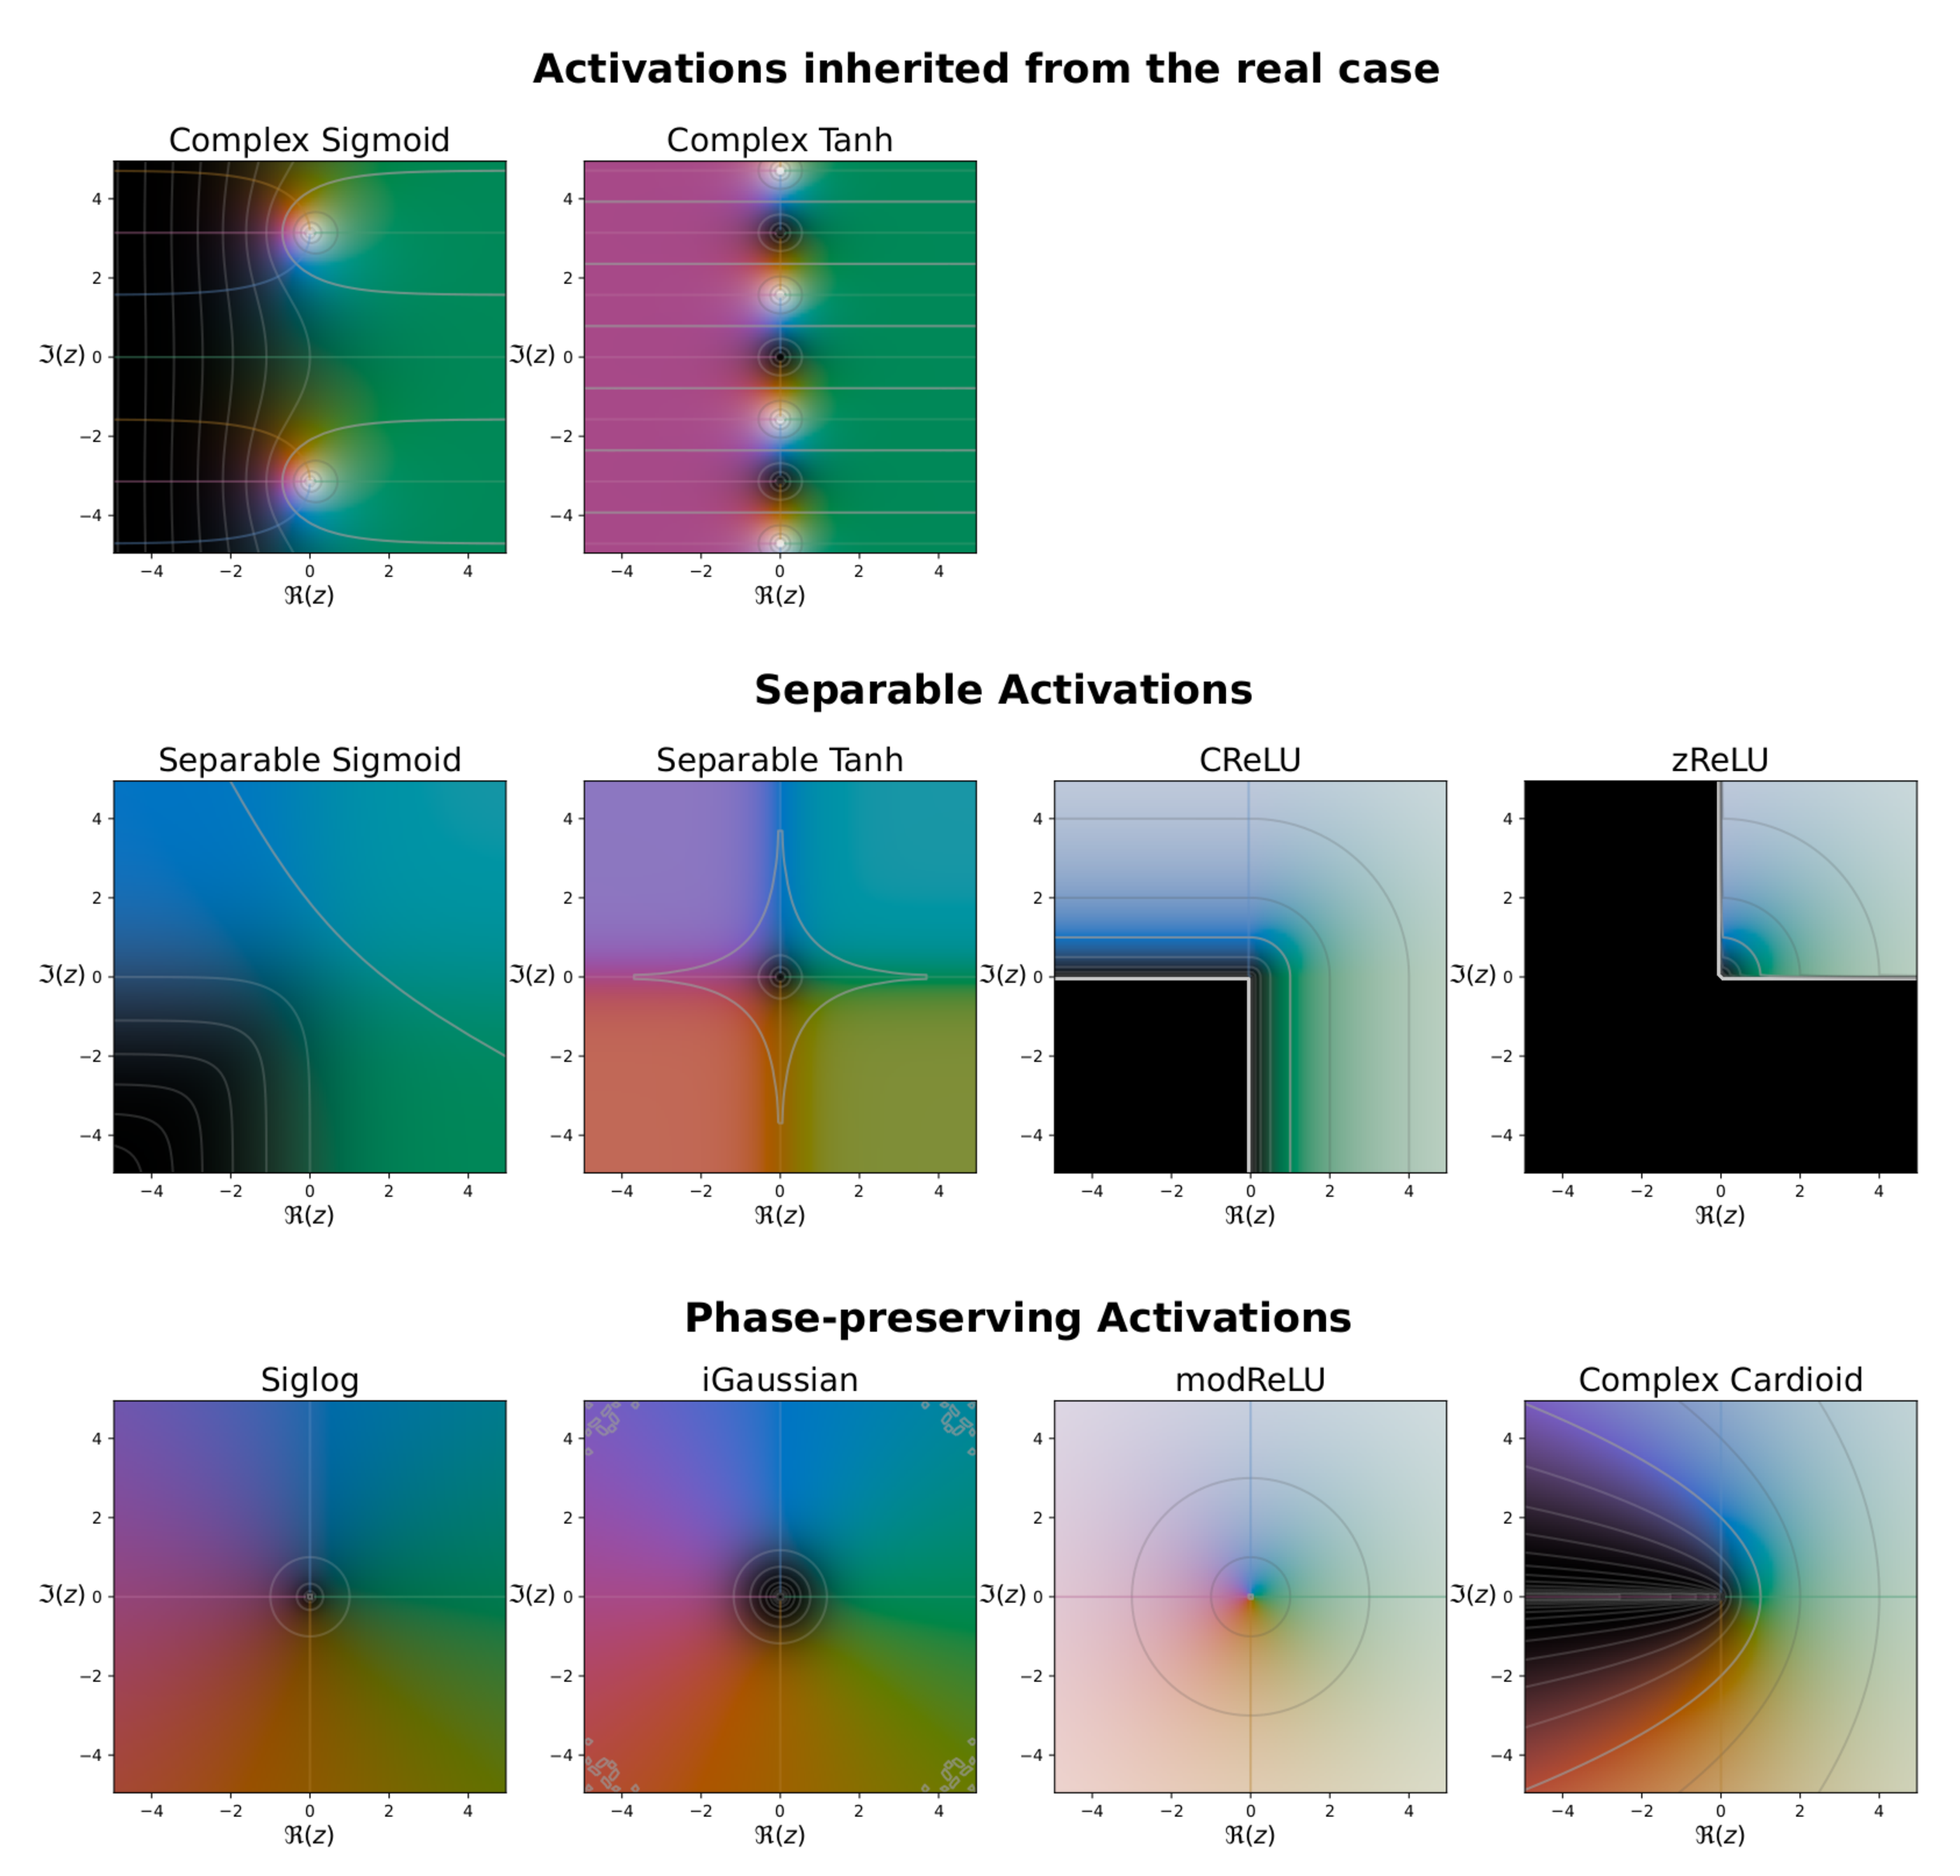
\includegraphics[width=0.9\textwidth]{pictures/cmplx_activations}
\end{figure}


\end{document}